\documentclass[runningheads]{llncs}
% Add pdf bookmarks.
\usepackage[bookmarksopen,bookmarksopenlevel=1,bookmarksdepth=2]{hyperref}
%
\usepackage{graphicx}
% If you use the hyperref package, please uncomment the following line
% to display URLs in blue roman font according to Springer's eBook style:
% \renewcommand\UrlFont{\color{blue}\rmfamily}

\usepackage{orcidlink} % Orcid links
% Fix underscore in dois
\usepackage[strings]{underscore}
% Modern tables
\usepackage{tabularray}
% Diagonal lines
\UseTblrLibrary{diagbox}

% Listing settings
\usepackage{listings}
\definecolor{DarkGreen}{HTML}{006400}

\lstdefinelanguage{BCoorLang}[]{Java}{
	basicstyle=\ttfamily,
    emph={
    	synchronize
    },
    commentstyle=\color{DarkGreen},
    emphstyle={\color{blue}\bfseries},
    numbers=left,
    numberstyle=\tiny\color{black},
}

\lstdefinelanguage{MontiArc}[]{Java}{
	basicstyle=\ttfamily,
	commentstyle=\color{DarkGreen},
	emph={
		component, port, automaton, initial, state, <<sync>>
	},
	alsoletter=<>,
	emphstyle={\color{blue}\bfseries},
	numbers=left,
	numberstyle=\tiny\color{black},
}

\begin{document}
% https://www.discotec.org/2024/coordination
% Regular papers 7-15 pages + references
% Artifacts using Zenodo together with this repo. Maybe a big CSV file with our classification results is input for some plots (clustering). Then, the source code for that should also be added.
% TODO: Make repo public and add artifacts citation using zenodo.
\title{A feature model for coordination approaches}
% Alternative titles:
% Comparing coordination approaches
% Comparing features coordination approaches
% Classifying coordination approaches
% Classifying features coordination approaches
% A feature model for coordination approaches
% How to coordinate? A feature model for coordination approaches
%
%\titlerunning{Abbreviated paper title}
% If the paper title is too long for the running head, you can set
% an abbreviated paper title here
%
\author{Tim Kr\"{a}uter\inst{1}\orcidlink{0000-0003-1795-0611} \and
Julien Deantoni\inst{2}\orcidlink{0000-0001-6962-7846}
Adrian Rutle\inst{1}\orcidlink{0000-0002-4158-1644} \and
Harald K\"{o}nig\inst{3,1}\orcidlink{0000-0001-6304-6311} \and
Yngve Lamo\inst{1}\orcidlink{0000-0001-9196-1779}}
%
\authorrunning{T. Kräuter et al.}
% First names are abbreviated in the running head.
% If there are more than two authors, 'et al.' is used.
\institute{Western Norway University of Applied Sciences, Bergen, Norway  \\
\email{tkra@hvl.no, aru@hvl.no, yla@hvl.no} \and
University Cote d’Azur, Sophia Antipolis, France \\
\email{julien.deantoni@univ-cotedazur.fr} \and
University of Applied Sciences, FHDW, Hanover, Germany\\
\email{harald.koenig@fhdw.de}}
%
\maketitle              % typeset the header of the contribution
%
\begin{abstract}
TODO
\keywords{
	Co-Simulation \and
	Coordination language \and
	ADL \and
	Coordination framework \and
	Feature model \and
	Taxonomy
}
\end{abstract}

\section{Introduction} \label{sec:introduction}

% Categorizing ADLs, Coordination languages, Co-simulation, and Coordination frameworks (BCOOL and me).

% Paper outline

% What was our search methodology? Google Scholar? Other databases? Which search terms/queries?
% ADL/Architecture description language & survey/classification/literature review

% Contribution
\textbf{Contribution.} We present a feature model comparing coordination approaches including coordination languages, ADLs, co-simulation tools, and coordination frameworks.

\section{Running example}
In this section, we introduce a running example that will be used throughout the paper to as an example to explain the different coordination approaches.
\autoref{fig:overviewRunningExample} depicts \textit{pedestrian crossing} the running example.

The example shows traffic lights (TLs) for cars and pedestrians.
To guarantee \textit{safe crossing} of pedestrians, the car TLs should be red when the pedestrian TLs are green and vice versa.
Thus, the car and pedestrian TLs cannot act independently, i.e., they must coordinate.
In addition, the car or pedestrian TLs must be green to ensure \textit{progress in traffic} flow.

\begin{figure}[ht]
	\centering
	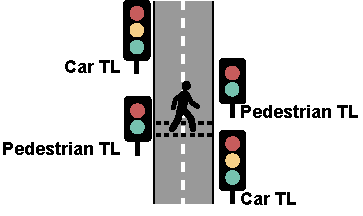
\includegraphics[width=0.5\textwidth]{images/running_example_schematic}
	\caption{Pedestrian crossing running example}
	\label{fig:overviewRunningExample}
\end{figure}

The behavior of the pedestrian TLs and car TLs are depicted as UML state machines \cite{objectmanagementgroupUnifiedModelingLanguage2017} in \autoref{fig:stateMachinesRunningExample}.

\begin{figure}[ht]
	\centering
	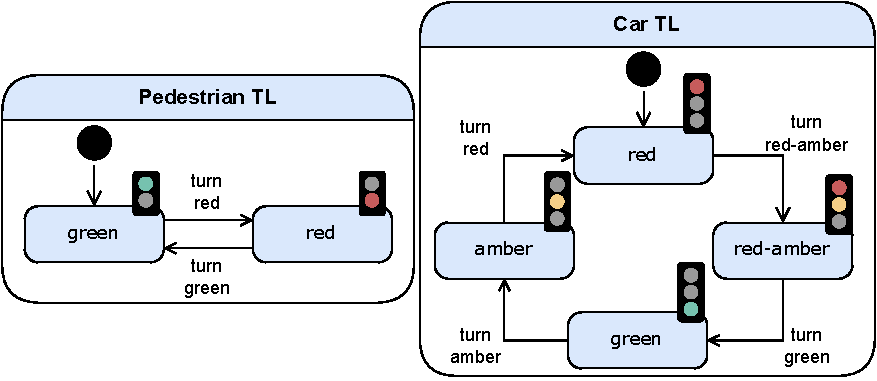
\includegraphics[width=1\textwidth]{images/running_example_models}
	\caption{Pedestrian TL and car TL as state machines}
	\label{fig:stateMachinesRunningExample}
\end{figure}

A \texttt{Pedestrian TL} can be \texttt{green} or \texttt{red}, while a \texttt{Car TL} has \texttt{red-amber} and \texttt{amber} as intermediate states between \texttt{red} and \texttt{green}.
How \textit{safe crossing} and \textit{progress in traffic} are achieved differs between the used coordination approaches.

The running example is deliberately kept simple because the focus should be on the coordination approaches, not the example's complexity.
Furthermore, the example does not need continuous variables and thus is not sufficient to show the full capabilities of Co-Simulation compared to the other coordination approaches.
However, since continuous variables from physical systems cannot be represented in all coordination approaches, we opted for this running example, which represents a minimal denominator between all coordination approaches and is familiar to everyday life.

\section{Categories of Coordination Approaches} \label{sec:approaches}

\autoref{fig:overview} gives an overview of the different categories of coordination approaches.
The first two categories of coordination approaches mostly focus on the \textit{execution} level, i.e., they operate directly with source code or executable binaries.

\textbf{Co-Simulation Tools} usually use the Functional Mock-up Interface (FMI)\footnote{\url{https://fmi-standard.org/}} standard, which defines executable systems parts, so-called Functional Mock-up Units (FMUs).
Each FMU consists of an executable and an XML model to describe its interface, for example, the FMU's exposed variables.
FMI is heavily used in the industry because it protects intellectual property (IP) since executables are black-box, i.e., do not expose implementation details.

\textbf{Coordination Languages} traditionally offer a shared tuple space for concurrent programs to read/write data from/to.
Separating \textit{coordination} from \textit{computation}, which seems natural today, was pioneered by coordination languages such as Linda \cite{carrieroLindaContext1989}.
% See if we can find a better citation for LF.
New coordination languages are being developed, such as Lingua Franca \cite{lohstrohReactorsDeterministicModel2020}, which use coordination mechanisms similar to ADLs but on the execution level.

\begin{figure}[ht]
	\centering
	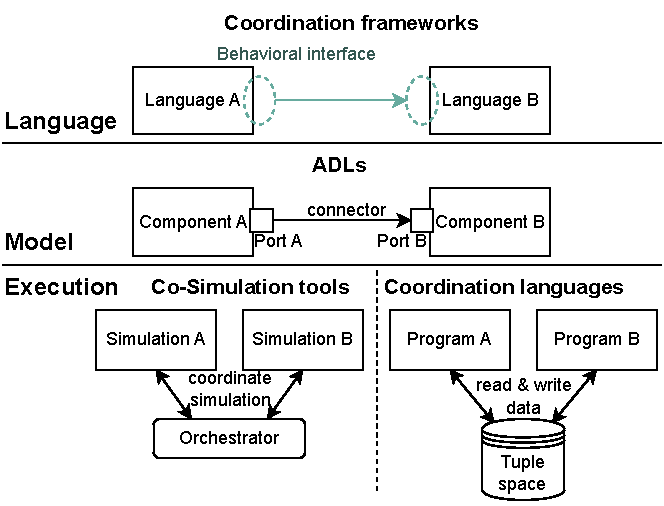
\includegraphics[width=0.7\textwidth]{images/overview}
	\caption{Overview of coordination approaches}
	\label{fig:overview}
\end{figure}

\textbf{Architecture Description Languages (ADLs)} operate on the \textit{model} level, i.e., each \textit{component} is given by a behavioral specification/model, for example, a state machine.
Components coordinate through \textit{connectors} between them, resulting in a \textit{architectural configuration}.

\textbf{Coordination frameworks} allow the user to connect models conforming to different behavioral languages using the concept of behavioral interfaces.
In contrast, each ADL usually only allows one behavioral language, which must be used for each component.
Thus, they operate on the \textit{language} level and give modelers freedom to utilize different languages for varying aspects of the system.

In the following sections, we will describe each category in detail.

\subsection{Architecture Description Languages} \label{subsec:adl}
% General idea
Architecture Description Languages (ADLs) aim to describe the structure of systems, allowing developers to focus on high-level components and their connections rather than lines of source code~\cite{clementsSurveyArchitectureDescription1996,medvidovicClassificationComparisonFramework2000,medvidovicFrameworkClassifyingComparing1997}.
% What is an ADL, and what is not?
Many different ADLs have been proposed in the academic literature and by the industry~\cite{medvidovicClassificationComparisonFramework2000,woodsArchitectureDescriptionLanguages2005}.
Nevertheless, clearly defining ADLs is challenging due to overlap with general-purpose modeling languages~\cite{clementsSurveyArchitectureDescription1996}.

% Describing ADLs generally.
The three buildings blocks of ADLs are defined as (1) \textit{components}, (2) \textit{connectors}, (3) \textit{architectural configuration}~\cite{medvidovicClassificationComparisonFramework2000,medvidovicFrameworkClassifyingComparing1997}.
% Component
A \textit{component} is a unit of computation or data repository~\cite{medvidovicClassificationComparisonFramework2000}.
Components vary in size, ranging from representing individual services to entire systems.

% Connector
\textit{Connectors} serve as architectural elements to model interactions between components and the regulations that oversee those interactions~\cite{medvidovicClassificationComparisonFramework2000}.
A difference to components is that connectors must not be implemented as distinct entities such as message brokers but can also represent shared variables or links between applications realized by client-server protocols \cite{medvidovicClassificationComparisonFramework2000}.

% Architectural configuration
\textit{Architectural configuration}, also known as topology, represents the structural arrangement of components and connectors in a connected graph, defining the overall architecture~\cite{medvidovicClassificationComparisonFramework2000}.
This structure determines if the combined semantics results in the desired behavior.
For example, one can check for deadlocks and starvation.

% ADLS are formal and usually incorporate one formal language. Usually, a process algebra. They do not support multiple formal specification languages cite medvidovicClassificationComparisonFramework2000.
In addition, ADLs incorporate a formal language to enable analysis.
The first ADLs usually use process algebras such as Communicating Sequential Processes (CSP), Calculus of Communicating Systems (CCS), and $\pi$-calculus \cite{ozkayaAreWeThere2013}.
For example, Wright uses CSP \cite{allenFormalBasisArchitectural1997} while Darwin uses $\pi$-calculus \cite{mageeSpecifyingDistributedSoftware1995}.
More recent ADLs, such as MontiArc \cite{haberMontiArcArchitecturalModeling2014}, use automata to define the behavior of components.

However, no ADL supports multiple formal languages such as the coordination frameworks discussed in \autoref{subsec:frameworks} \cite{medvidovicClassificationComparisonFramework2000}.
Furthermore, despite the creation of numerous ADLs in the literature, they are not mainstream, i.e., used often by practitioners in the industry \cite{clementsSurveyArchitectureDescription1996,woodsArchitectureDescriptionLanguages2005,pandeyArchitecturalDescriptionLanguages2010,ozkayaAreWeThere2013}.

For this paper, we consider only ADLs that incorporate formal semantics and thus do not consider other modeling languages such as UML \cite{objectmanagementgroupUnifiedModelingLanguage2017} and ArchiMate \cite{theopengroupArchiMateSpecification2023} despite them being sometimes seen as ADLs and their usage in the industry.

A representative example of an ADL is given in  \autoref{lst:MontiArc-Crossing} showing the \textit{components} for the pedestrian crossing running example in MontiArc.

\lstinputlisting[
label=lst:MontiArc-Crossing,
language=MontiArc,
caption=MontiArc component for the pedestrian crossing]{listings/MontiArc-PedestrianCrossing.arc}

It defines three components: \textsf{PedestrianCrossing}, \textsf{PedestrianTL}, and \textsf{CarTL}.
Furthermore, the components \textsf{PedestrianTL} and \textsf{CarTL} define ports (line 10 and 15).
The \textit{architectural configuration} is defined in the \textsf{PedestrianCrossing} component (lines 1-7), which links the ports of the \textsf{PedestrianTL} and \textsf{CarTL} using a \textit{connector} (line 6).
The behavior of the \textsf{PedestrianTL} and \textsf{CarTL} component is omitted but given later in \autoref{subsec:montiArc}.

\subsection{Coordination Languages}
% Define Coordination language and give examples
% Cite and survey

\subsection{Co-Simulation Tools}
% Define Co-Simulation and give examples
\cite{gomesCoSimulationSurvey2019} % co-simulation survey

% Rewrite this part
Co-simulation aims to solve this challenge by composing the simulation of a system's parts into a global simulation \cite{gomesCoSimulationSurvey2019}.

For example, \cite{ekerTamingHeterogeneityPtolemy2003} propose an actor-oriented co-simulation approach, where each system part is represented as an actor.
An actor can communicate through its interfaces with other actors.
Their approach is implemented in the tool \textit{Ptolemy} and supports continuous time and state variables.
% FMI/FMU standard
Furthermore, the Functional Mock-up Interface (FMI)\footnote{\url{https://fmi-standard.org/}} is a co-simulation standard to exchange executable systems parts, so-called Functional Mock-up Units (FMUs).
Each FMU, similar to the actors in Ptolemy, comes with an XML model to describe its interface, for example, the FMU's exposed variables.
FMUs support continuous time and state variables and are widely used in the industry.

However, with co-simulations, one can only simulate systems, not check global behavioral properties.

\subsection{Coordination Frameworks} \label{subsec:frameworks}
% Define Coordination-framework and give examples
% Surveys? Probably not.

% Distinguishing factors
The main differences between coordination frameworks and ADLs are as follows.

\textbf{(1) Heterogeneous models:} Coordination frameworks do not mandate one behavioral language or formalism for every model.
One can pick the most suitable language or formalism for each part of the system supported by the coordination framework.
For example, the car TL in the running example could be defined using a different behavioral language such as a UML activity diagram \cite{objectmanagementgroupUnifiedModelingLanguage2017}, a BPMN process model \cite{objectmanagementgroupBusinessProcessModel2013}, or a $\pi$-calculus term \cite{milnerCommunicatingMobileSystems2010}.

% Behavioral interfaces
\textbf{(2) Behavioral interfaces:} To coordinate between heterogeneous models \textit{behavioral interfaces} are used.
These interfaces are defined for each language or generally for all languages and represent a common understanding, which is needed when each language can be different.
Examples of coordination frameworks are Behavioral Coordination Operator Language (BCOoL) \cite{varalarsenBCOolBehavioralCoordination2016,varalarsenBehavioralCoordinationOperator2015} and BCoorLang \cite{krauterBehavioralConsistencyMultimodeling2023}.
% Ptolemy?

% BCoorLang is the new name. A bit close to BCOoL.
For example, using BCoorLang, one would define a \textit{system relationship model}, see \autoref{fig:exampleBCoorLang}, which defines existing behavioral models and their relations similar to the architectural configuration of ADLs.

\begin{figure}[ht]
	\centering
	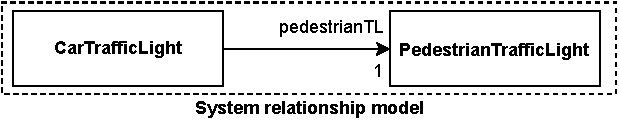
\includegraphics[width=0.7\textwidth]{images/running_example_BCorrLang}
	\caption{System relationship model for the running example}
	\label{fig:exampleBCoorLang}
\end{figure}

Using the behavioral relationship between \textsf{CarTrafficLight} and \textsf{PedestrianTrafficLight}, one can then define synchronizations of their behavior.
To describe the behavior of car TL and pedestrian TL, one can use the state machines defined in the running example (see \autoref{fig:stateMachinesRunningExample}) since the state machine behavioral language is supported in BCoorLang \cite{krauterBehavioralConsistencyMultimodeling2023}.


\section{Feature model} \label{sec:features}
% Add some kind of introduction: Coordination approaches have only been analyzed separatly (cite studies co-simulation, adl, something about coordinatino languages) but never compared/aligned in the broader context.
% We try to find overlaps and unique features (differntiators) between the different approaches.

The feature model for coordination approaches is shown in \autoref{fig:featureModelOverview} where each coordination approach has three main feature sets: \textit{Coordination}, \textit{Goal}, and \textit{Properties}.

\begin{figure}[ht]
	\centering
	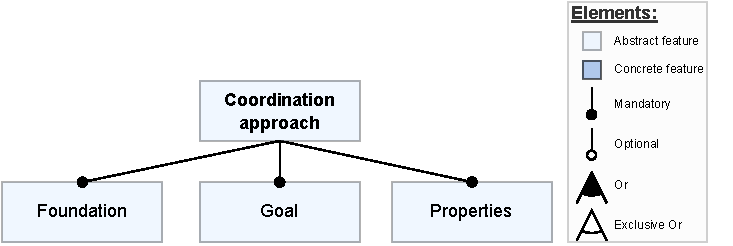
\includegraphics[width=0.8\textwidth]{images/root}
	\caption{Feature model overview}
	\label{fig:featureModelOverview}
\end{figure}

In the following sections, we will describe each feature set in detail.
% TODO: Add the full feature model as an artifact (at the end when the feature model is stable).
A complete diagram of the feature model is contained in \cite{timkrauterArtifactsCoordination2024}.

% TODO: Make this section more readable. Better examples, explanations and linking of paragraphs.
\subsection{Coordination}

\autoref{fig:coordinationFeature} shows the \textbf {Coordination} feature, which consists of \textbf{Definition}, \textbf{Elements of coordination}, and \textbf{Semantics}.

% Maybe cut into two pieces. So, Definition and Semantics are not part of the same.
\begin{figure}[ht]
	\centering
	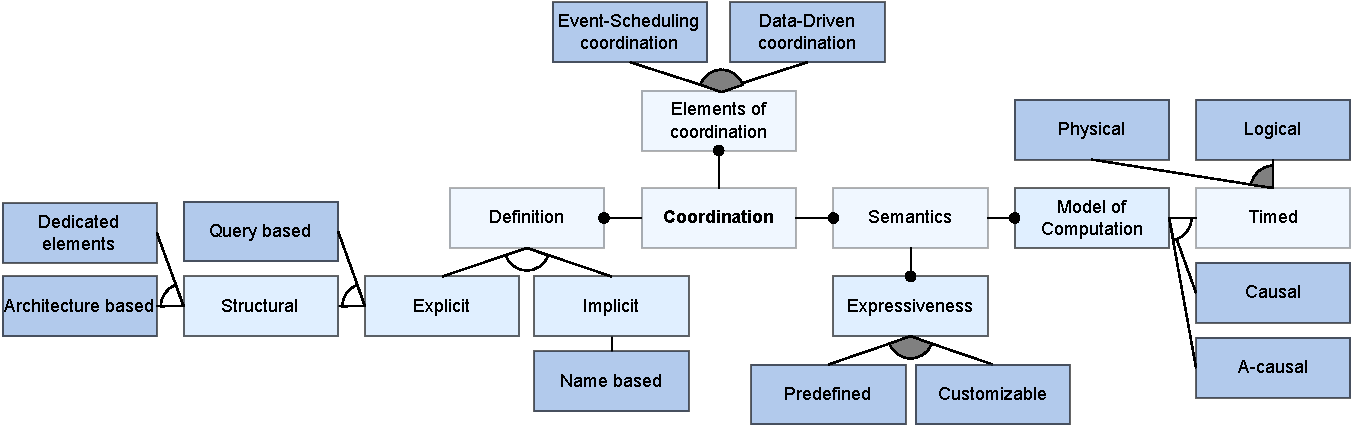
\includegraphics[width=1\textwidth]{images/coordination_feature}
	\caption{Coordination feature}
	\label{fig:coordinationFeature}
\end{figure}

\textbf{Definition} The definition of coordination can either be \textit{explicit} or \textit{implicit}.
Implicit definition is usually based on the names of model elements.
For example, one could synchronize transitions of state machines if they have identical names.

Explicit definition is either \textit{query based} or \textit{structural}.
% Query-based example
For example, in BCOoL \cite{varalarsenBCOolBehavioralCoordination2016,varalarsenBehavioralCoordinationOperator2015}, one can write expressions to define which elements should coordinate.

A structural definition of coordination uses \textit{dedicated elements} or is \textit{architecture based}.
For example, interactions in BCoorLang are specified by dedicated elements, while coordination in ADLs depends on the architectural configuration \cite{medvidovicClassificationComparisonFramework2000}, i.e., how ports of components are connected.

\textbf{Elements of coordination} The main elements driving coordination can be events, data, or both.
\textit{Event-scheduling coordination}, used in BCOoL and BCoorLang, orders or synchronizes events/state changes in different models.
\textit{Data-driven coordination} is used in Co-Simulation where components send data to input ports or even directly change variables other components expose.

\textbf{Semantics} The semantics feature consists of \textit{expressiveness} and \textit{model of computation}.
The expressiveness of coordination can be \textit{predefined}, i.e., a user has a fixed set of coordination mechanisms or \textit{customizable}.
For example, in BCOoL, the user can employ the Clock Constraints Specification Language (CCSL) \cite{andreSyntaxSemanticsClock2009} when defining coordination \cite{varalarsenBCOolBehavioralCoordination2016,varalarsenBehavioralCoordinationOperator2015}.

Coordination approaches utilize different \textit{models of computation} (MoC).
% What is a model of computation? Where does the terminology come from?
% causal a-causal also identified as causality in gomesCoSimulationSurvey2019
We define three MoCs: \textit{timed}, \textit{causal}, \textit{a-causal}, where \textit{timed} is either \textit{physical} or \textit{logical}.
% We should define that event and state-changing elements mean the same, i.e., any observable action in a model/component.
% Causal (events and data)
The causal MoC means that the coordination approach can define \textit{causal} relationships between events of different components.
For example, a transition in a state machine raises an event that causes a reaction in an activity diagram due to the defined coordination.
% A-causal
A-causal MoC are employed in Co-Simulation, which can deal with sets of differential equations.
For example, a variable in one equation should be equal to a variable in a different equation.
One variable does not cause the other to change they should just be equal.

% Timed::Logical
\textit{Logical} time means that coordination approaches define when events/state changes happen.
Typically, one defines that events take place simultaneously or that one event causes another event or causes another event with a fixed delay.
For example, a delay could be 50 milliseconds of logical time, which corresponds to time in a simulation that can run arbitrarily fast. 
% Timed::Physical --> other term wall-clock time see gomesCoSimulationSurvey2019 and its citations
In contrast, \textit{physical} time describes time passing in the physical world.
One can, for example, define that one event should happen 50 milliseconds after another event.
In Lingua Franca \cite{lohstrohReactorsDeterministicModel2020}, logical time "chases" physical time, i.e., logical time tries to match the physical time provided by the execution platform.
% Logical time, however, always lags behind physical time.


\subsection{Goal} % Or even call it motivation
We identified three different \textit{goals} of coordination approaches: \textbf{coordinated simulation}, \textbf{coordinated execution}, and \textbf{formal verification}, see \autoref{fig:goalFeature}.
Usually approaches focus on one goal, for example co-simulation tools provide a coordinated simulation, while others such as coordination frameworks might provide formal verification in addition to simulation.
However, which types of dynamic systems can be simulated varies and is discussed in the next section.

\begin{figure}[ht]
	\centering
	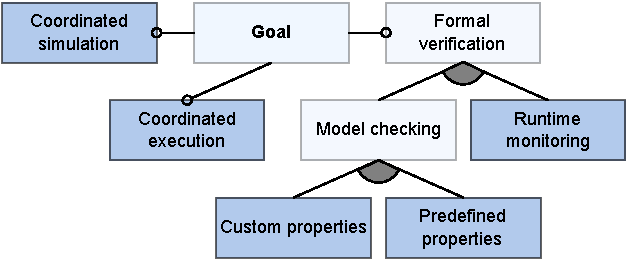
\includegraphics[width=0.7\textwidth]{images/goal_feature}
	\caption{Goal feature}
	\label{fig:goalFeature}
\end{figure}

% TODO: Introduce somewhere that component is equal to the behavioral model. Or means the same.
\textbf{Coordinated simulation} The most common goal of coordination approaches is a coordinated simulation of multiple components or behavioral models representing the entire system.
A coordinated simulation is useful because the composition of multiple components can lead to unexpected behavior, often called \textit{emergent behavior} \cite{ekerTamingHeterogeneityPtolemy2003}.
Emergent behavior can then be dealt with early in the development process before implementing each component and its interactions.
Co-simulation tools are an example of approaches that have coordinated simulation as their goal.

\textbf{Coordinated execution} In contrast to coordinated simulation, which often only aims to find errors, the goal of coordination approaches such as coordination languages is a coordinated execution.
Approaches with this goal are not only used during development but also provide coordination capabilities when a composite system is deployed and executed in a production setting.

\textbf{Formal verification} Another goal of coordination approaches, especially for safety-critical systems, is formal verification.
Formal verification can be used before the system is deployed (\textit{model checking}) or while it is running (\textit{runtime monitoring}).



For model checking, we found coordination approaches that check \textit{predefined properties} or \textit{custom properties}.
% Wright is checking deadlock freedom of component interactions, i.e., connectors. (Definition 5)
For example, the ADL Wright \cite{allenFormalBasisArchitectural1997} can check \textit{deadlock freedom} of component interactions.
% Darwin and we are checking custom properties: mageeBehaviourAnalysisSoftware1999 krauterBehavioralConsistencyMultimodeling2023
The coordination framework in \cite{krauterBehavioralConsistencyMultimodeling2023}

\subsection{Properties}
% Categorization corresponds to the different co-simulation approaches described in gomesCoSimulationSurvey2019.
We identified several common \textit{properties} when analyzing coordination approaches, see \autoref{fig:propertiesFeature}.

\begin{figure}[ht]
	\centering
	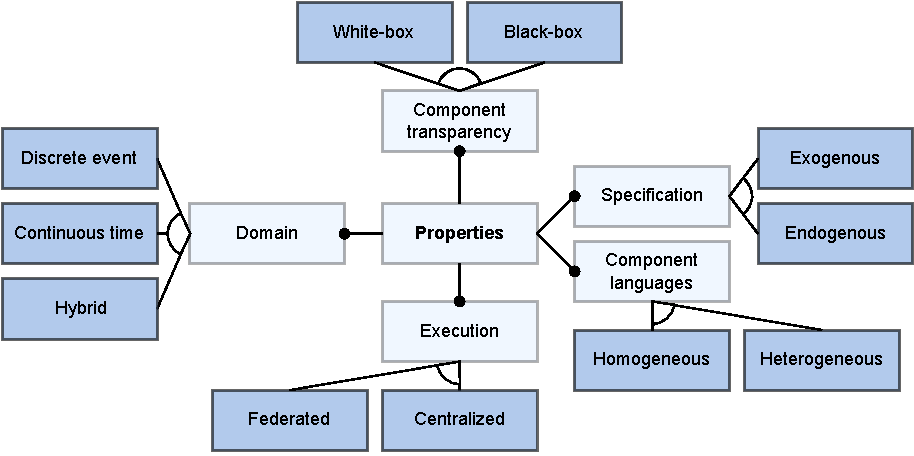
\includegraphics[width=1\textwidth]{images/properties_feature}
	\caption{Properties feature}
	\label{fig:propertiesFeature}
\end{figure}

% Maybe add some examples and description here.
\textbf{Domain} Coordination approaches operate in different domains, similar to the categorization of co-simulation approaches in \cite{gomesCoSimulationSurvey2019}.
\textit{Discrete event} means a coordination approach assumes discrete state changes, while in the \textit{continuous time} domain variables can be continuous due to differential equations.
In a \textit{hybrid} domain both discrete and continuous variables are mixed.

The choice of a coordination approach is dependent on the nature of the system at hand.
For instance, software systems usually can be modeled in the discrete event domain, while physical or cyber-physical systems operate in the continuous time or even hybrid domain.

% Should be clear from earlier that component is a program or behavioral model.
\textbf{Coordination specification} Coordination can either be defined inside components (\textit{intrusive}), i.e., one has to change the component or outside of components (\textit{non-intrusive}).


\textbf{Component languages} Coordination languages typically only support coordination of if each component is written in the same programming language (\textit{homogeneous}).
Similarly, most ADLs only coordinate components defined using the same modeling language.
However, coordination frameworks typically allow components specified in different behavioral languages (\textit{heterogeneous}).


\textbf{Implementation} Coordination approaches can be implemented as a \textit{co-simulation} where.
% insert co-simulation here. Master algorithm or something.
An alternative is a \textit{unified execution} either using the same underlying \textit{programming language} or \textit{formal language}.
Coordination frameworks typically convert heterogeneous components to a common formal language.


\section{Classification} \label{sec:classifications}
\autoref{tab:classification} shows the classification of four different coordination approaches.
% TODO: Add a citation for each approach
Each approach represents a co-simulation tool (\textit{DACCOSIM}), coordination language (\textit{Linda}), ADL (\textit{MontiArc}), or coordination framework (\textit{BCoorLang}).
However, we classified more than just the four representatives chosen.
All classification are available in the artifacts of this paper \cite{timkrauterArtifactsCoordination2024}.

% Could even have two tables for better sizing and maybe adding 1-2 approaches.
% TODO: Double check DACCOSIM and make sure it is the best co-simulation pick.
\begin{table}
	\centering
	\caption{Approach classification}
	\label{tab:classification}
	\resizebox{\textwidth}{!}{
	\begin{tblr}{
			column{2-Z} = {c},
			rows = {5mm},
			hline{1, 2, Z} = {-}{1.2pt, solid}, % Z is the last row/column
			hline{7, 11} = {-}{dashed},
			vline{2-Y} = {2-Z}{solid},
		}
		\diagbox[linewidth=1.1pt, width=4.4cm,font=\bfseries]{Feature}{Approach} & BCoorLang & Linda & MontiArc & DACCOSIM \\
		
		\textbf{Coordination} \\
		\hspace{2mm} Definition & Dedicated elements & Name based & Architecture based & Name based \\
		\hspace{2mm} Elements of coordination & Event-Scheduling & Data-driven & Data-driven & Data-driven \\ % everything ends in coordination here in the feature model
		\hspace{2mm} Expressiveness & Predefined & Predefined & Predefined & Predefined \\
		\hspace{2mm} MoC & Timed:Logical & Causal & Timed:Logical, Causal & Causal \\
		
		\textbf{Goal} \\
		\hspace{2mm} Coordinated simulation & + & - & + & - \\
		\hspace{2mm} Coordinated execution & - & + & - & + \\
		\hspace{2mm} Formal verification & Custom properties & - & - & - \\
		
		\textbf{Properties} \\
		\hspace{2mm} Domain & Discrete event & Discrete event & Discrete event & Hybrid \\
		\hspace{2mm} Coordination specification & Non-intrusive & Intrusive & Intrusive & Intrusive \\
		\hspace{2mm} Component languages & Heterogeneous & Homogeneous & Homogeneous & Homogeneous \\	
		\hspace{2mm} Implementation & Formal language & PL & PL & PL \\
	\end{tblr}
	}
\end{table}

\subsection{BCoorLang}
First, we will explain BCoorLang by implementing the running example and then we classify it using our feature model.

\textbf{Running example:} In BCoorLang there are two fundamental concepts: \textit{state} and \textit{state-changing elements}, which must be defined for each behavioral language.
For state machines, these are defined in \cite{krauterBehavioralConsistencyMultimodeling2023}.
State-changing elements act as a uniform behavioral interface to define interactions between heterogeneous models.

\autoref{lst:interactions} shows how the synchronizations required by the running example can be implemented as \textit{interactions} in BCoorLang.
The interactions use the system relationship model defined earlier in \autoref{fig:exampleBCoorLang} and synchronize specific transitions in the state machines.
Transitions are the state-changing elements in state machines, see  \cite{krauterBehavioralConsistencyMultimodeling2023}.

\lstinputlisting[
label=lst:interactions,
language=BCoorLang,
caption=Interactions for the running example]{listings/BCoordLang.txt}

\autoref{lst:interactions} synchronizes the turning red of the car TL with the turning green of the pedestrian TL and vice versa.
The individual models and interactions are then transformed into a behavioral specification for the global system.
% Overkill if there is only one behavioral language.
The transformation might result in a graph transformation (GT) system.
Using model checking supported by GT tools proves that the two requirements \textit{safe crossing} and \textit{progress in traffic} are fulfilled by synchronization.
% TODO: Add executable GT with a tutorial to the artifacts. Maybe also Maude one.
The executable GT specification for the running example can be found in \cite{timkrauterArtifactsCoordination2024}.

\textbf{Classification:} 

\subsection{MontiArc} \label{subsec:montiArc}
First, we will explain MontiArc by implementing the running example and then classify it using our feature model.

\textbf{Running example:} To implement the example, we define a component for the \textsf{PedestrianCrossing} with two subcomponents for each type of TL.
The pedestrian crossing component is already defined in \autoref{lst:MontiArc-Crossing} in \autoref{subsec:adl}.

The \textsf{CarTL} component is active.
It controls the passive \textsf{PedestrianTL} component by sending events through its output port, which is bound to the input port of the \textsf{PedestrianTL}, see the configuration in \autoref{lst:MontiArc-Crossing}.
\autoref{lst:MontiArc-PTL} shows the \textsf{CarTL} component.

\lstinputlisting[
label=lst:MontiArc-PTL,
language=MontiArc,
caption=MontiArc component for the car TL.]{listings/MontiArc-CarTL.arc}

The \textsf{PedestrianTL} component waits for signals coming through its port to change its state.
Thus, it is controlled by the events sent by the \textsf{CarTL} component.
\autoref{lst:MontiArc-CTL} shows the \textsf{PedestrianTL} component.

\lstinputlisting[
label=lst:MontiArc-CTL,
language=MontiArc,
caption=MontiArc component for the pedestrian TL.]{listings/MontiArc-PedestrianTL.arc}

Synchronization of the two components is achieved due to the ports being synchronized.
This means, transitions that send and receive events through these ports are executed atomically.
Thus, when the \textsf{CarTL} switches to \textsf{Green}, the \textsf{PedestrianTL} switches to \textsf{Red} and vice versa.

Inspecting the execution trace when running the implementation for 20 steps indicates that the two requirements \textit{safe crossing} and \textit{progress in traffic} are fulfilled by the synchronization.
The executable source code of the MontiArc implementation for the running example can be found in \cite{timkrauterArtifactsCoordination2024}.

% TODO: Describe the classification here!
\textbf{Classification:} bla
\subsection{Lingua Franca/Linda} % Coordination language representative
\subsection{Co-Simulation example} % Co-Simulation representative
\subsection{BCOOL} % Coordination framework representative

\section{Findings} % or Classification results --> Interprete the previous classification
% Clusters of features for ADL, Coordination language, Co-Simulation, and coordination frameworks?
% Maybe they can somehow be visualized nicely using some clusters with overlaps (vann diagram or something)

% Commonalities between clusters

% Differences between clusters

% What are the unique features of each approach? Does this match their intended usage scenarios?

\section{Conclusion} \label{sec:conclusion}

\bibliographystyle{splncs04}
\bibliography{bib}

\end{document}
